\graphicspath{{content/chapters/4_results/figures/}}

\chapter{Results and Discussion}%
\label{chp:results}

\section{Replication}%
\label{sec:replication}

As mentioned in Section~\ref{sec:implementation}, each model considered was
evaluated on a dataset used by the original authors to verify it was replicated
correctly. As noted in Section~\ref{sec:datasets} the supervised models were
evaluated on the CSE-CIC-IDS2018 dataset whilst the unsupervised models were
evaluated on the NSL-KDD dataset. The evaluation methodology was also evaluated
on the models and dataset originally used by Kus et al.~\cite{Kus}.
Tables~\ref{tab:karatas_rep_agg} and~\ref{tab:karatas_rep_acc} display the
results of the replication of the work of Karatas et al.~\cite{Karatas}.
%
\begin{table}
    \caption{Karatas et al.~\cite{Karatas} replication aggregate results\label{tab:karatas_rep_agg}}
    \centering
    \begin{tblr}{|c|c|c|c|c|c|c|}
        \hline
        \textbf{Algorithm} & \textbf{Accuracy}  & \textbf{Recall}
                           & \textbf{Precision} & \textbf{F1-Measure} \\
        \hline
        \gls{dt}           & 0.99               & 0.97
                           & 0.94               & 0.95                \\
        \gls{rf}           & 0.99               & 0.94
                           & 0.95               & 0.95                \\
        \gls{gb}           & 0.99               & 1.00
                           & 0.96               & 0.98                \\
        \gls{knn}          & 0.97               & 0.91
                           & 0.71               & 0.76                \\
        \gls{lda}          & 0.88               & 0.89
                           & 0.52               & 0.57                \\
        \hline
    \end{tblr}
\end{table}
%
\begin{table}
    \caption{Karatas et al.~\cite{Karatas} replication accuracy per class\label{tab:karatas_rep_acc}}
    \centering
    \begin{tblr}{|c|c|c|c|c|c|c|}
        \hline
        \textbf{Algorithm} & \textbf{Benign}      & \textbf{Bot}       &
        \textbf{\gls{dos}} & \textbf{Brute Force} & \textbf{Injection} &
        \textbf{Infiltration}                                                  \\
        \hline
        \gls{dt}           & 0.993                & 1.000              & 1.000
                           & 1.000                & 0.805              & 1.000 \\
        \gls{rf}           & 0.991                & 1.000              & 1.000
                           & 1.000                & 0.747              & 0.917 \\
        \gls{gb}           & 0.991                & 1.000              & 1.000
                           & 1.000                & 0.987              & 1.000 \\
        \gls{knn}          & 0.970                & 1.000              & 1.000
                           & 1.000                & 0.490              & 1.000 \\
        \gls{lda}          & 0.840                & 1.000              & 1.000
                           & 0.961                & 0.626              & 0.917 \\
        \hline
    \end{tblr}
\end{table}
%
Table~\ref{tab:cao_rep} shows the results of the replication of the work of Cao
et al.~\cite{Cao}.
%
\begin{table}
    \caption{Cao et al.~\cite{Cao} replication \gls{auc} per class\label{tab:cao_rep}}
    \centering
    \begin{tblr}{|c|c|c|c|c|c|c|}
        \hline
        \textbf{Algorithm}    & \textbf{Benign} & \textbf{Probe} &
        \textbf{\gls{dos}}    & \textbf{R2L}    & \textbf{U2R}
        \\
        \hline
        \gls{sae}-\gls{ocsvm} & 0.962           & 0.975          & 0.972
                              & 0.926           & 0.959
        \\
        \hline
    \end{tblr}
\end{table}
%
Figures~\ref{fig:kus_rep_exc} and~\ref{fig:kus_rep_inc} show the results of the
replication of the work of Kus et al.~\cite{Kus}. The results present metrics
employed by the original authors, that were considered in order to verify the
works were replicated correctly. Note, the label encodings used by our
replication of the work of Kus et al.~\cite{Kus} is different to that of the
original authors, hence, the columns of the heatmaps appear to be shuffled. The
encoding zero represents the benign class in both our replication and the
original work.
%
\begin{figure}[htbp]
    \centering
    \begin{minipage}[h]{0.5\textwidth}
        \centering
        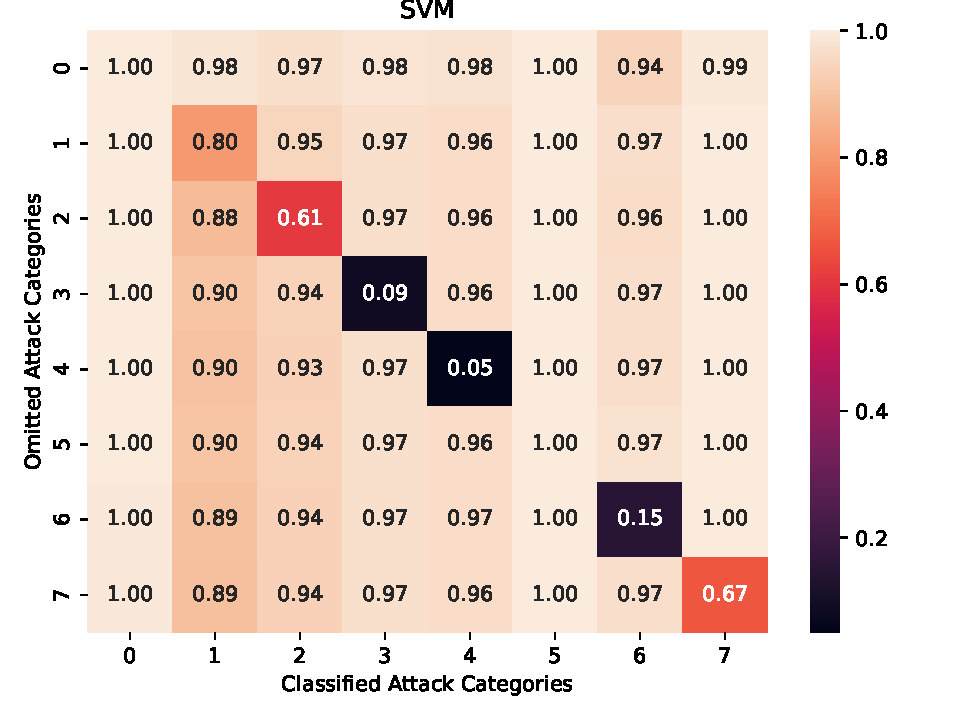
\includegraphics[width=\textwidth,keepaspectratio]{kus_rf_exc_category}
    \end{minipage}\hfill
    \begin{minipage}[h]{0.5\textwidth}
        \centering
        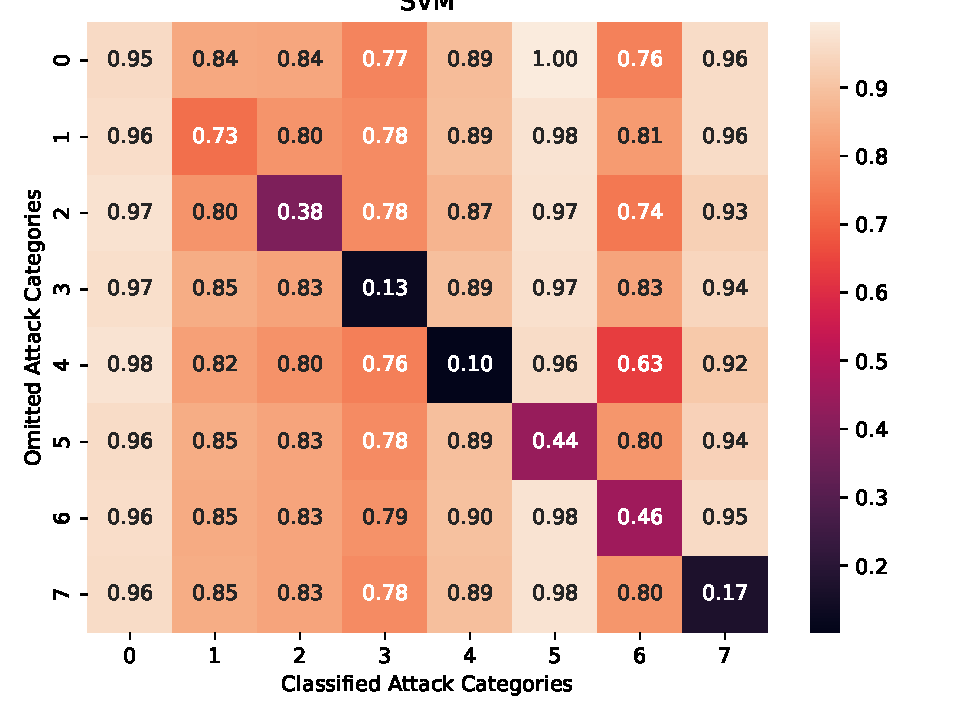
\includegraphics[width=\textwidth,keepaspectratio]{kus_svm_exc_category}
    \end{minipage}
    %
    \begin{minipage}[h]{0.5\textwidth}
        \centering
        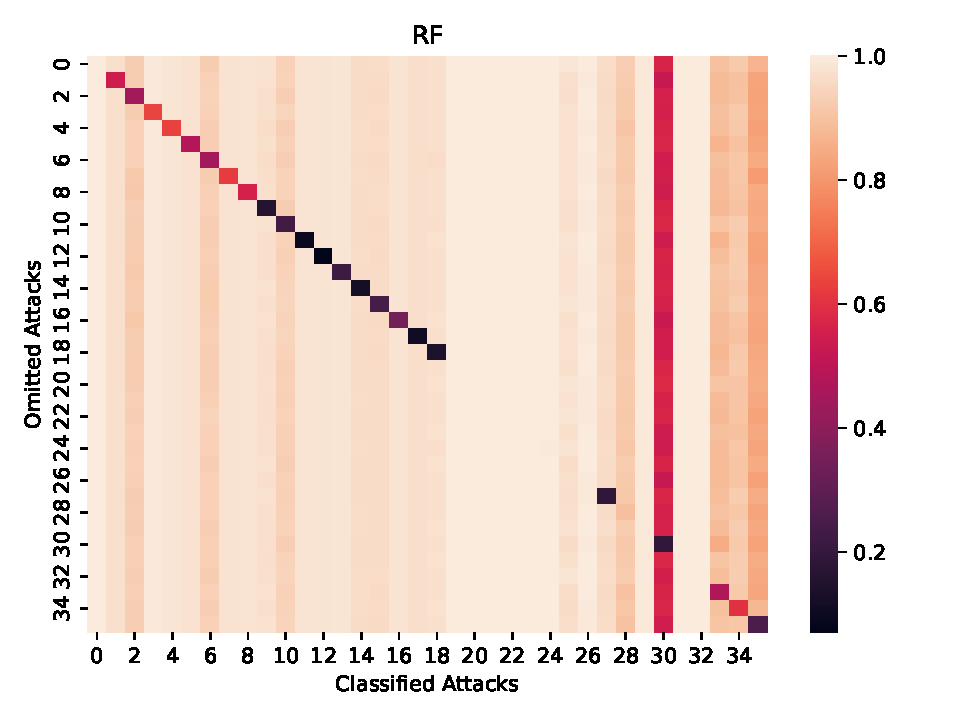
\includegraphics[width=\textwidth,keepaspectratio]{kus_rf_exc_attack}
    \end{minipage}\hfill
    \begin{minipage}[h]{0.5\textwidth}
        \centering
        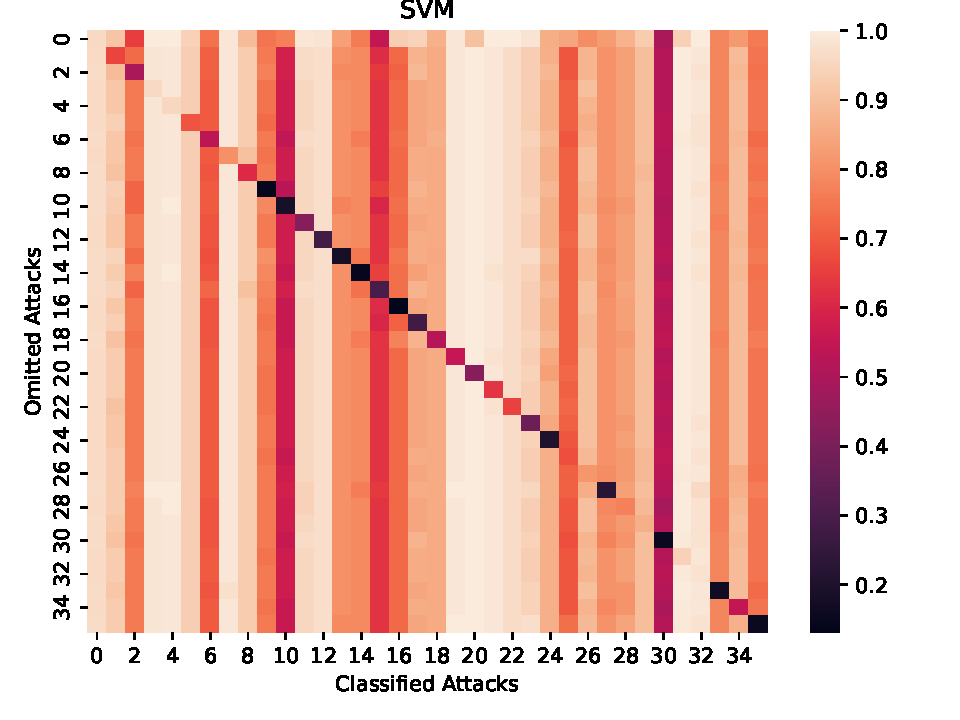
\includegraphics[width=\textwidth,keepaspectratio]{kus_svm_exc_attack}
    \end{minipage}
    \caption[Kus et al.~\cite{Kus} Replication Class Omission Heatmaps]{Kus et al.~\cite{Kus} replication heatmaps illustrating recall per class against omitted class\label{fig:kus_rep_exc}}
\end{figure}

\begin{figure}[htbp]
    \centering
    \begin{minipage}[h]{0.5\textwidth}
        \centering
        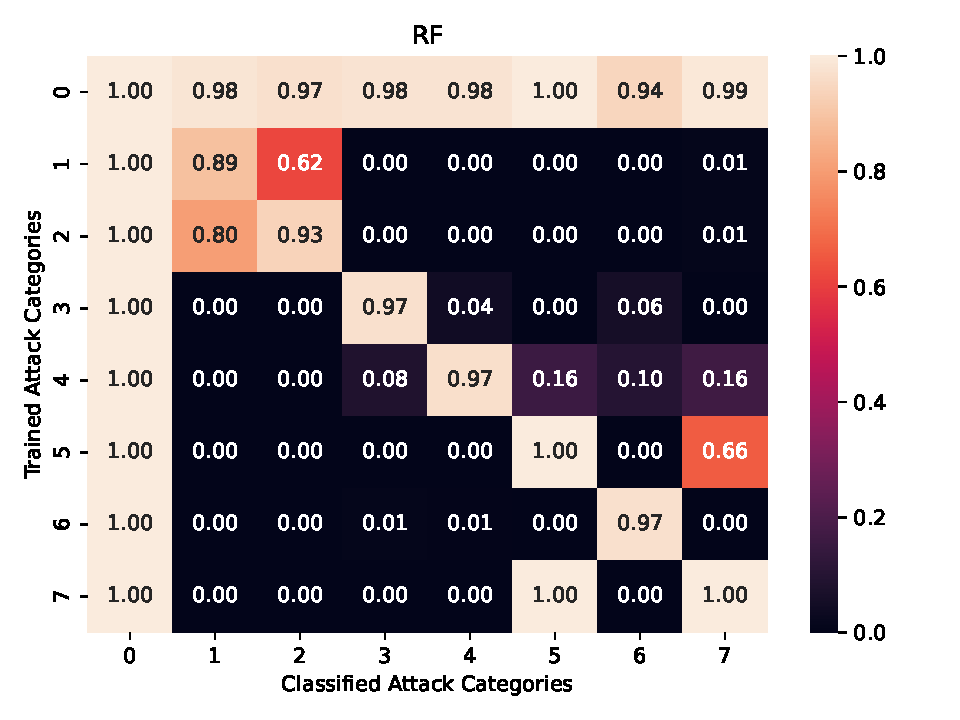
\includegraphics[width=\textwidth,keepaspectratio]{kus_rf_inc_category}
    \end{minipage}\hfill
    \begin{minipage}[h]{0.5\textwidth}
        \centering
        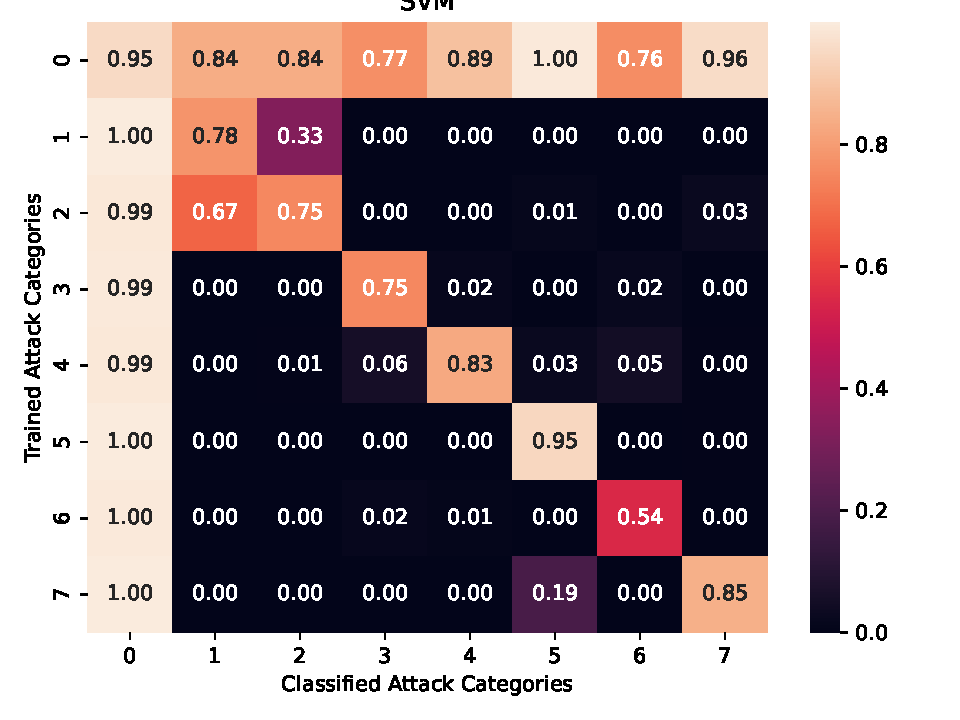
\includegraphics[width=\textwidth,keepaspectratio]{kus_svm_inc_category}
    \end{minipage}
    %
    \begin{minipage}[h]{0.5\textwidth}
        \centering
        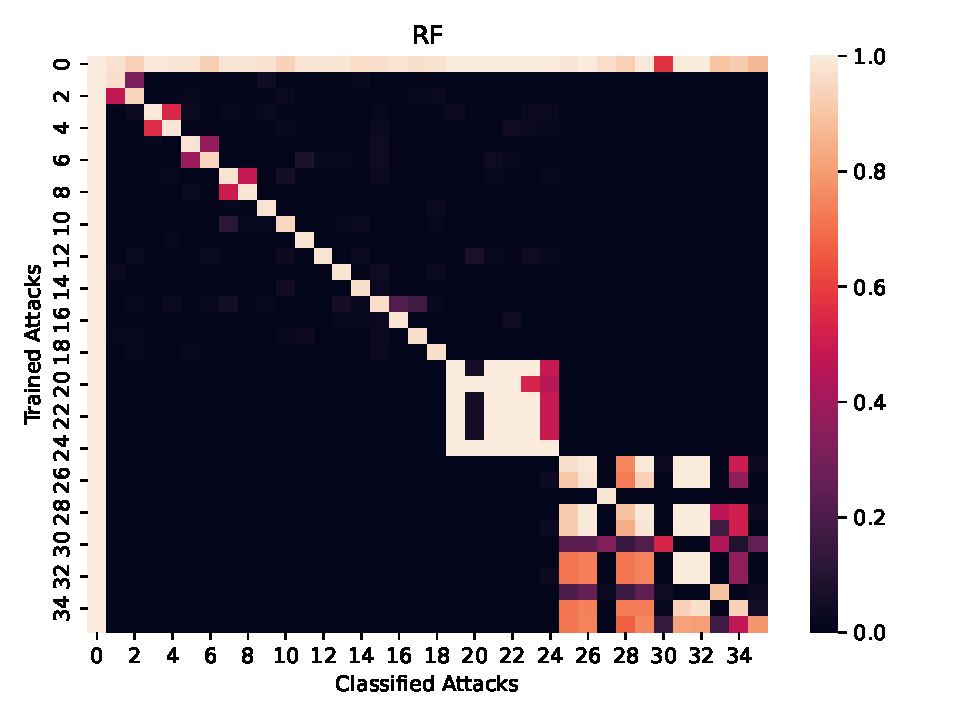
\includegraphics[width=\textwidth,keepaspectratio]{kus_rf_inc_attack}
    \end{minipage}\hfill
    \begin{minipage}[h]{0.5\textwidth}
        \centering
        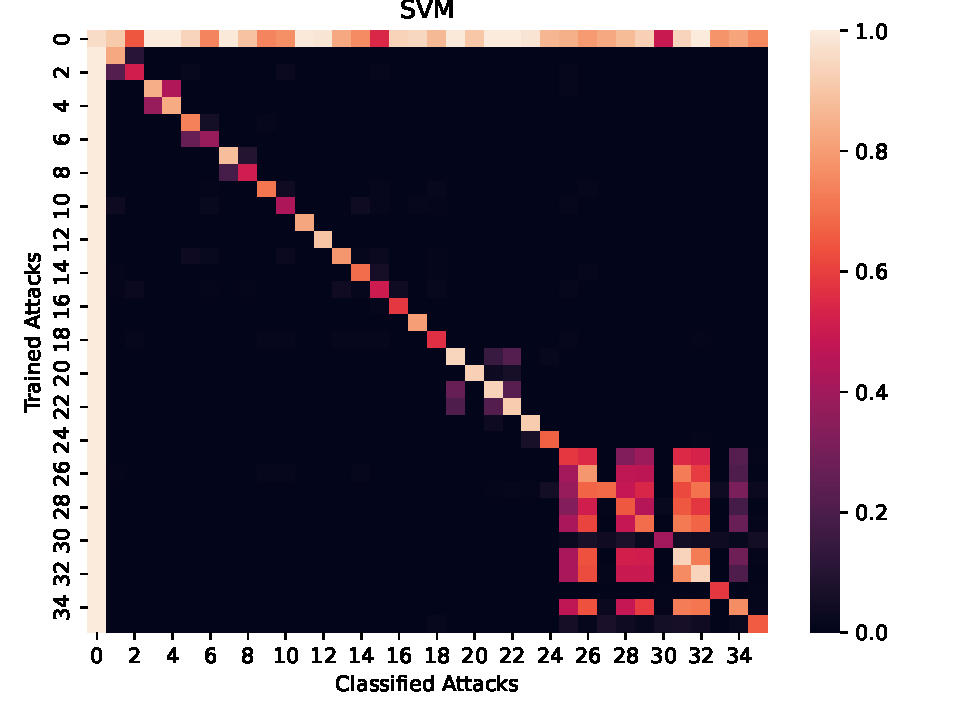
\includegraphics[width=\textwidth,keepaspectratio]{kus_svm_inc_attack}
    \end{minipage}
    \caption[Kus et al.~\cite{Kus} Replication Single Class Heatmaps]{Kus et al.~\cite{Kus} replication heatmaps illustrating recall per class against trained class\label{fig:kus_rep_inc}}
\end{figure}
% 

\section{Aggregate Results Omitting Categories}%
\label{sec:agg_res_cat}

% TODO: add unsupervised heatmaps

The aggregate results of all the experiments are shown in
Table~\ref{tab:results_cat_agg}. The results shown for the supervised models
are the averages of the metrics generated from the first phase of training
variants, which each have one attack category excluded. These variants were
selected to generate the aggregate results as they offer the most realistic
simulation of a practical scenario whereby an unknown attack is deployed on a
model trained on several categories of known attacks. The macro-average was
taken when aggregating across classes to reduce the impact of class imbalance.
The recall-unk column indicates the average recall of each variant, taking into
account only the excluded category.

% category
\begin{table}
    \caption{Aggregate results when excluding
        categories\label{tab:results_cat_agg}}
    \centering
    \begin{tblr}{|c|c|c|c|c|c|c|}
        \hline
        \textbf{Algorithm}    & \textbf{Accuracy}  & \textbf{Recall}     &
        \textbf{Recall-Unk}   & \textbf{Precision} & \textbf{F1-Measure}         \\
        \hline
        \gls{dt}              & 0.962              & 0.828               & 0.134
                              & 0.942              & 0.832                       \\
        \gls{rf}              & 0.964              & 0.830               & 0.228
                              & 0.910              & 0.848                       \\
        \gls{gb}              & 0.948              & 0.804               & 0.118
                              & 0.872              & 0.800                       \\
        \gls{knn}             & 0.958              & 0.800               & 0.248
                              & 0.900              & 0.796                       \\
        \gls{lda}             & 0.914              & 0.766               & 0.564
                              & 0.850              & 0.718                       \\
        \gls{ssc}-\gls{ocsvm} & 0.760              & 0.590               & 0.554
                              & 0.820              & 0.670                       \\
        \gls{sae}-\gls{ocsvm} & 0.800              & 0.640               & 0.600
                              & 0.830              & 0.650                       \\ % & 0.825 (AUC)
        \hline
    \end{tblr}
\end{table}

The results of the supervised models are generally high indicating a good
ability to detect known attacks from network data, with the \gls{dt} and
\gls{rf} algorithms performing slightly better than the \gls{gb} algorithm.
However, this degrades significantly in the face of unknown attacks. This is
indicated by the low values in the recall-unk column, with \gls{rf} performing
better than the other two models, however still very poorly. This indicates a
very low ability to generalise to unknown attack categories in these models.

The unsupervised model on the other hand exhibits a negligible difference
between its recall and recall-unk values, however has a lower recall value than
the supervised models. The accuracy and F1-score of the model is also lower
indicating worse overall performance when compared to the supervised models.
The accuracy stands at 80\% which is a notable figure, however, as previously
mentioned, the accuracy may be skewed by a large number of correct benign
predictions. Hence, the recall and F1-score may be more significant given the
class imbalance present in the dataset. Considering the recall and F1-score in
Table~\ref{tab:results_cat_agg}, the \gls{sae}-\gls{ocsvm} model does not
demonstrate a high efficacy in network intrusion detection, only successfully
identifying 64\% of attacks.

From these observations, we can begin to address \hyperlink{obj}{Objective 1}.
The state-of-the-art supervised models considered demonstrate impressive
efficacy in detecting known network intrusions, however, their efficacy
diminishes to an alarming degree when faced with unknown attacks. Hence, their
overall efficacy will depend on the types of attacks the system is expected to
face, and the dataset available for training. The state-of-the-art unsupervised
model considered exhibits a far lower efficacy, however, experiences negligible
decline against unknown attacks. This may offer an invaluable tool in flagging
potentially malicious behaviour however, may not be suitable if a high degree
of confidence in predictions is required. Regarding \hyperlink{obj}{Objective
    2}, it is clear to see that the supervised models considered are more effective
overall, performing better in all metrics except for recall-unk. However,
unsupervised models are significantly more effective in detecting unknown
attacks.

\begin{table}
    \caption{Accuracy per class when excluding
        categories\label{tab:results_cat_acc}}
    \centering
    \begin{tblr}{|c|c|c|c|c|c|c|}
        \hline
        \textbf{Algorithm}    & \textbf{Benign}      & \textbf{Bot}       &
        \textbf{\gls{dos}}    & \textbf{Brute Force} & \textbf{Injection} &
        \textbf{Infiltration}                                                     \\
        \hline
        \gls{dt}              & 0.990                & 0.971              & 0.849
                              & 0.902                & 0.938              & 0.440 \\
        \gls{rf}              & 0.994                & 0.802              & 0.815
                              & 0.902                & 0.862              & 0.448 \\
        \gls{gb}              & 0.989                & 0.741              & 0.622
                              & 0.751                & 0.754              & 0.240 \\
        \gls{knn}             & 0.985                & 0.801              & 0.831
                              & 0.920                & 0.892              & 0.388 \\
        \gls{lda}             & 0.940                & 0.773              & 0.805
                              & 0.951                & 0.954              & 0.162 \\
        \gls{ssc}-\gls{ocsvm} & 0.772                & 0.006              & 0.778
                              & 0.999                & 0.667              & 0.313 \\
        \gls{sae}-\gls{ocsvm} & 0.818                & 0.496              & 0.734
                              & 0.999                & 0.384              & 0.391 \\
        \hline
    \end{tblr}
\end{table}

\begin{table}
    \caption{F1-Measure per class when excluding
        categories\label{tab:results_cat_f1}}
    \centering
    \begin{tblr}{|c|c|c|c|c|c|c|}
        \hline
        \textbf{Algorithm}    & \textbf{Benign}      & \textbf{Bot}       &
        \textbf{\gls{dos}}    & \textbf{Brute Force} & \textbf{Injection} &
        \textbf{Infiltration}                                                     \\
        \hline
        \gls{dt}              & 0.978                & 0.734              & 0.878
                              & 0.936                & 0.964              & 0.568
        \\
        \gls{rf}              & 0.978                & 0.670              & 0.828
                              & 0.936                & 0.894              & 0.576
        \\
        \gls{gb}              & 0.962                & 0.508              & 0.644
                              & 0.772                & 0.774              & 0.368
        \\
        \gls{knn}             & 0.974                & 0.554              & 0.856
                              & 0.950                & 0.926              & 0.522
        \\
        \gls{lda}             & 0.948                & 0.252              & 0.892
                              & 0.972                & 0.974              & 0.276
        \\
        \gls{ssc}-\gls{ocsvm} & 0.850                & 0.000              & 0.880
                              & 1.000                & 0.800              & 0.480
        \\
        \gls{sae}-\gls{ocsvm} & 0.870                & 0.070              & 0.850
                              & 1.000                & 0.560              & 0.560
        \\
        \hline
    \end{tblr}
\end{table}

Table~\ref{tab:results_cat_acc} includes the aggregate per class accuracy
calculated by averaging the per class accuracies of each variant where an
attack category is omitted. Table~\ref{tab:results_cat_f1} contains the per
class F1-scores averaged across the same variants.

Analysing the results of these tables, we can further investigate the behaviour
of the models. Firstly, we note that some attack categories appear to be harder
to predict than others. The Infiltration category for instance exhibits lower
accuracy across all models. A potential explanation for this is that
infiltration is a broad category involving the exploitation of software that
can take a wide variety of forms. Hence, infiltration attacks may differ
significantly among themselves making it harder for the model to learn common
patterns. Additionally, the dataset only contains five attacks under this
category, with a relatively small number of instances compared to most other
categories, potentially worsening the issue. Another potential explanation may
be that infiltration attacks resemble benign traffic more closely than other
categories, rendering themselves difficult to distinguish from normal traffic.

The comparison of the unsupervised model with the supervised models in
Table~\ref{tab:results_cat_acc} and Table~\ref{tab:results_cat_f1} reveals an
interesting phenomenon. Whilst the unsupervised model performs far worse
overall, it seems to perform very similarly to the supervised models on certain
categories. The model exhibits low efficacy on the DoS and Injection categories
specifically, weighing down its averages in the overall results. This is an
interesting observation as this means unsupervised models could serve as very
effective tool against both known and unknown attacks of specific categories,
against which it is known to be effective. Additionally, this finding brings
into question the reasons for this difference in performance. One potential
explanation is that these categories resemble benign traffic more closely
making it difficult to recognise them as anomalies, however, this hypothesis
would require further experimentation to confirm or deny concretely.

\section{Aggregate Results Omitting Specific Attacks}%
\label{sec:agg_res_att}
% attacks
\begin{table}
    \caption{Aggregate results when excluding specific
        attacks\label{tab:results_att_agg}}
    \centering
    \begin{tblr}{|c|c|c|c|c|c|c|}
        \hline
        \textbf{Algorithm}    & \textbf{Accuracy}  & \textbf{Recall}     &
        \textbf{Recall-Unk}   & \textbf{Precision} & \textbf{F1-Measure}         \\
        \hline
        \gls{dt}              & 0.981              & 0.870               & 0.465
                              & 0.960              & 0.884                       \\
        \gls{rf}              & 0.985              & 0.877               & 0.506
                              & 0.977              & 0.895                       \\
        \gls{gb}              & 0.980              & 0.830               & 0.546
                              & 0.966              & 0.842                       \\
        \gls{knn}             & 0.975              & 0.851               & 0.500
                              & 0.970              & 0.860                       \\
        \gls{lda}             & 0.918              & 0.758               & 0.610
                              & 0.958              & 0.767                       \\
        \gls{ssc}-\gls{ocsvm} & 0.760              & 0.630               & 0.566
                              & 0.900              & 0.690                       \\
        \gls{sae}-\gls{ocsvm} & 0.800              & 0.640               & 0.600
                              & 0.830              & 0.650                       \\
        \hline
    \end{tblr}
\end{table}

Table~\ref{tab:results_att_agg} shows the aggregate metrics from phase 1 of the
methodology, which involves excluding individual attacks to generate variants.
Similarly to Table~\ref{tab:results_cat_agg}, the macro average is taken across
classes to avoid overstating the results of the benign class.

The primary point to note from these results is the higher values found in the
recall-unk column. The supervised model, while still failing to match the
generalisation ability of the unsupervised model, perform far better than when
the entire category if omitted. This indicates these models are capable of
generalising to similar attacks and perform better on unknown attacks when
attacks in the same category are present in the dataset. However, as previously
mentioned, this generalisation ability is limited and still fails to supersede
that of the unsupervised model.

\section{Per Variant Results}%
\label{sec:res_var}

In this section, we will present and discuss heatmaps showing the recall values
on each category for each variant considered. This data will allow us to
address \hyperlink{obj}{Objective 3}, revealing the exact relationships each
model forms between the presence of attacks or attack categories in the
training set, and the predictions of each class.

%
\begin{figure}[htbp]
    \centering
    \begin{minipage}[h]{0.5\textwidth}
        \centering
        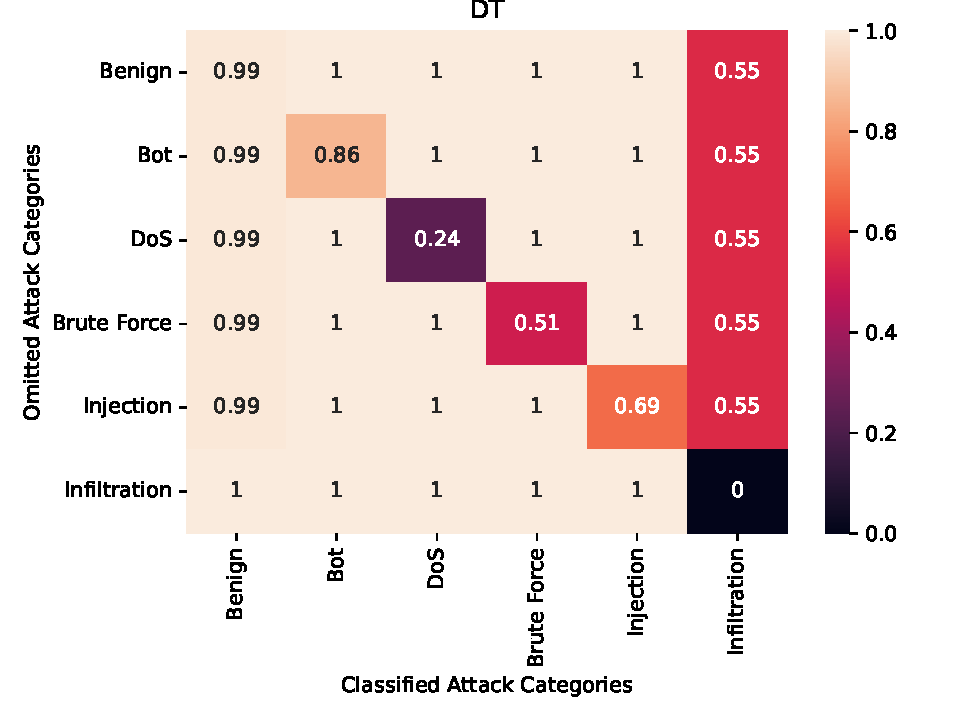
\includegraphics[width=\textwidth,keepaspectratio]{dt_exc_category}
    \end{minipage}\hfill
    \begin{minipage}[h]{0.5\textwidth}
        \centering
        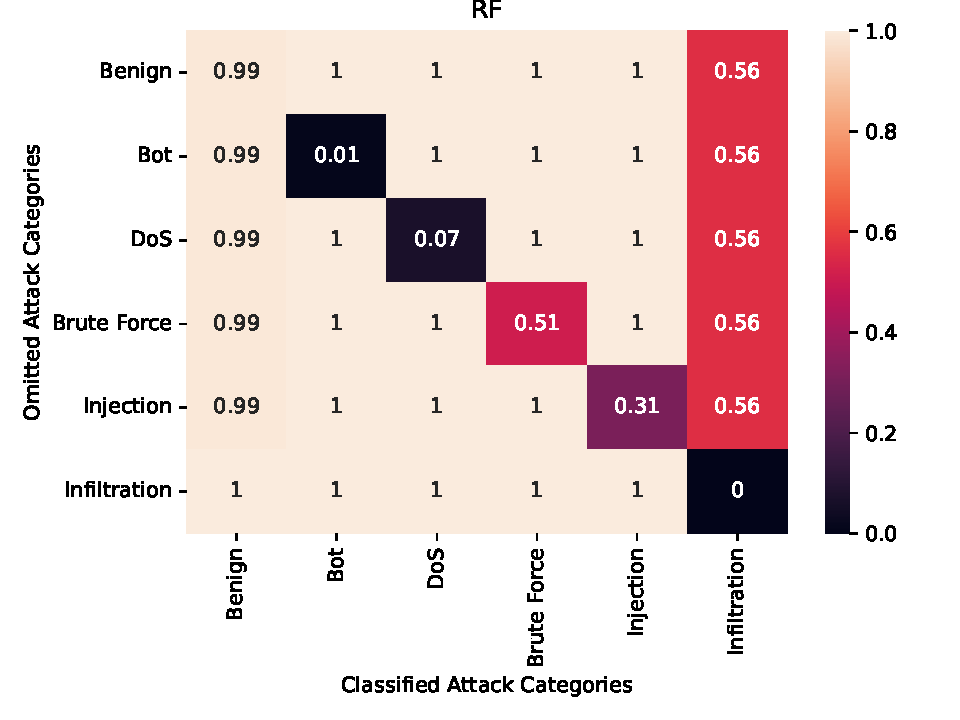
\includegraphics[width=\textwidth,keepaspectratio]{rf_exc_category}
    \end{minipage}
    %
    \begin{minipage}[h]{0.5\textwidth}
        \centering
        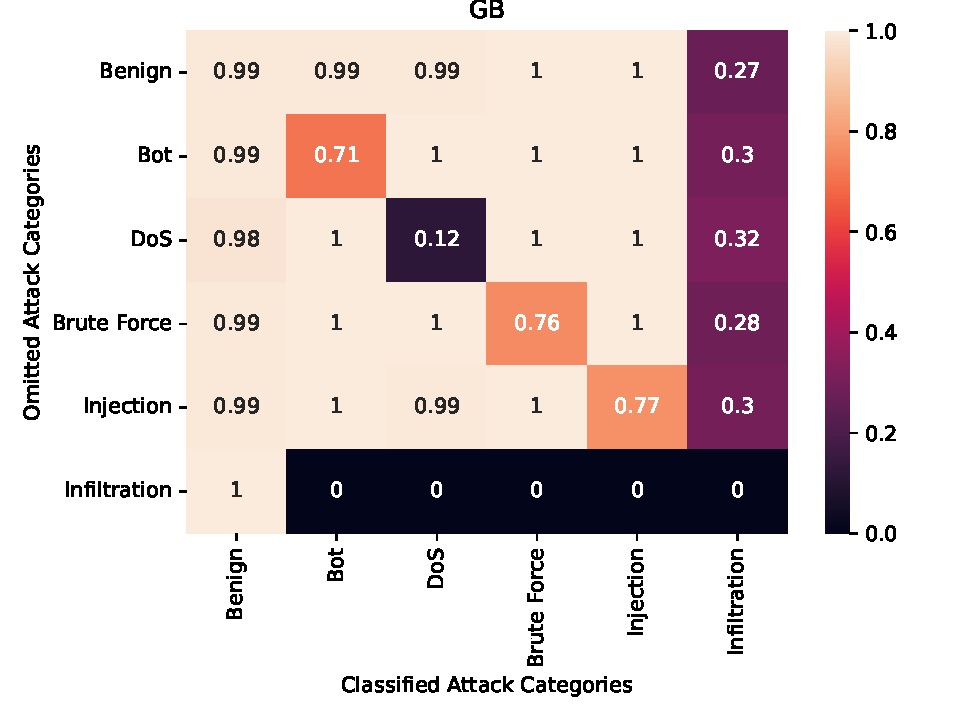
\includegraphics[width=\textwidth,keepaspectratio]{gb_exc_category}
    \end{minipage}\hfill
    \begin{minipage}[h]{0.5\textwidth}
        \centering
        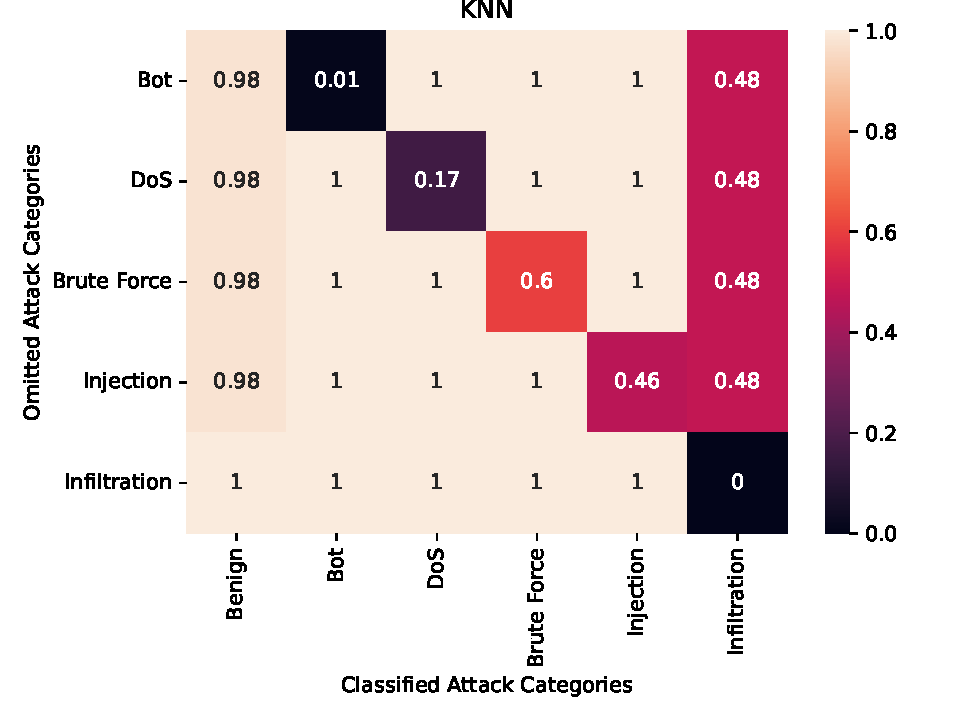
\includegraphics[width=\textwidth,keepaspectratio]{knn_exc_category}
    \end{minipage}
    \begin{minipage}[h]{0.5\textwidth}
        \centering
        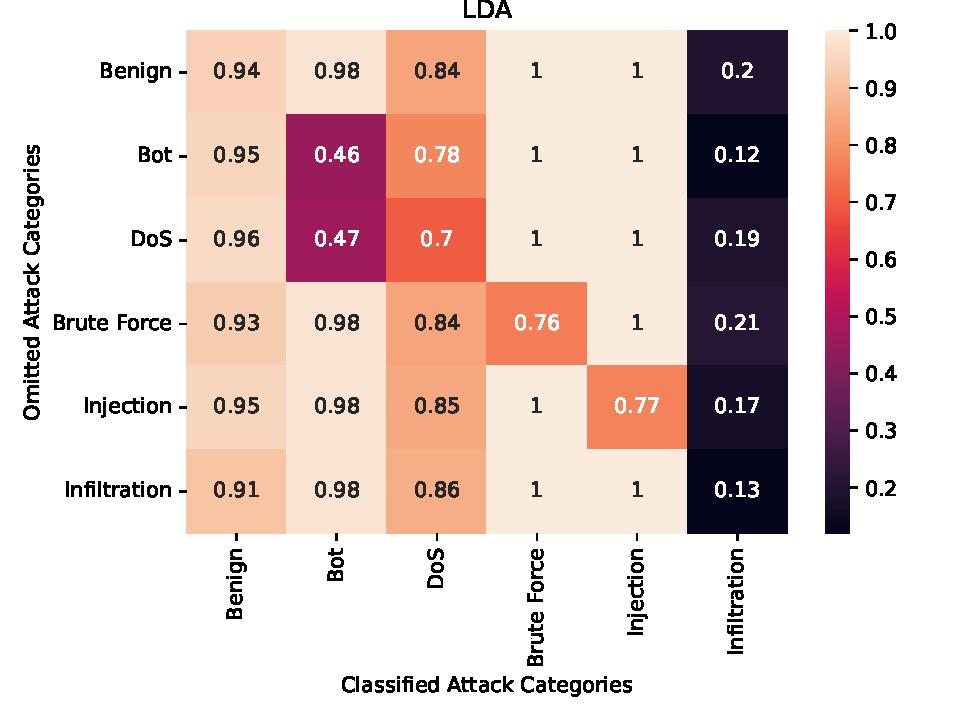
\includegraphics[width=\textwidth,keepaspectratio]{lda_exc_category}
    \end{minipage}
    \caption[Category Omission Results]{Recall values per class when trained on variants omitting a single category.\label{fig:exc_cat}}
\end{figure}
% 
Figure~\ref{fig:exc_cat} shows the heatmaps of recall values of the supervised
models generated from the variants omitting categories. Each row represents the
per category recall values generated from one variant. The label of the row is
the category that was omitted.

The results in these heatmaps further confirm the observations made earlier on
the high efficacy of supervised models on known attacks and reduced efficacy on
unknown attacks. Based on the recall values in the diagonals, the \gls{dt}
algorithm seems to generalise to unknown categories better than the \gls{rf}
algorithm. The \gls{gb} algorithm shows interesting behaviour as it seems to be
dependent on the infiltration category to learn patterns on the other classes,
achieving zero recall values when the category is excluded. Paradoxically, the
algorithm also exhibits the lowest infiltration recall of the models.
%
\begin{figure}[htbp]
    \centering
    \begin{minipage}[h]{0.5\textwidth}
        \centering
        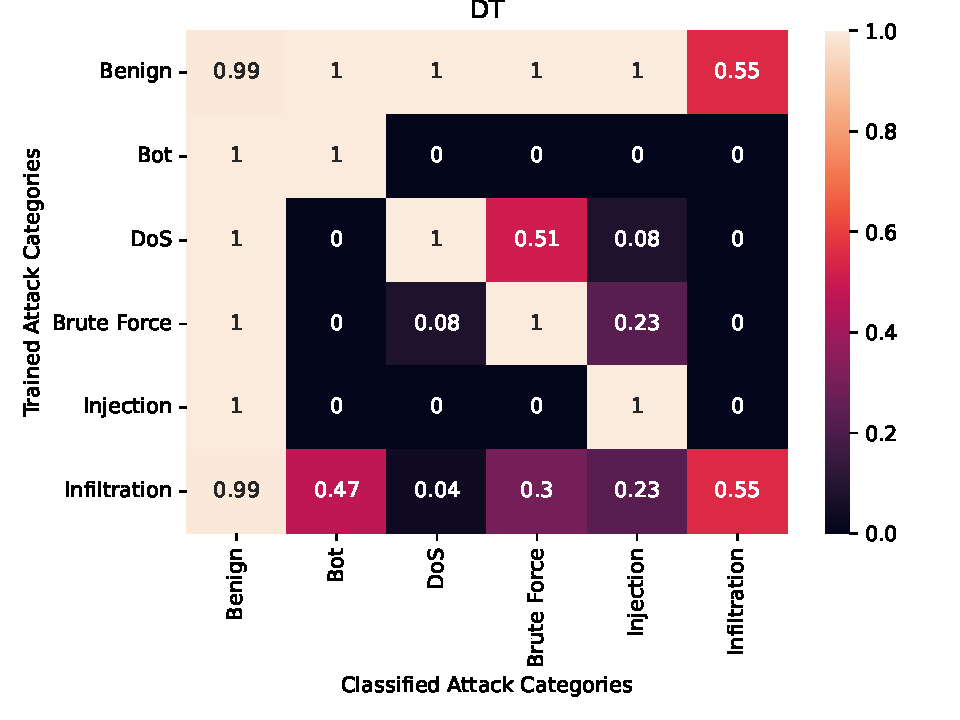
\includegraphics[width=\textwidth,keepaspectratio]{dt_inc_category}
    \end{minipage}\hfill
    \begin{minipage}[h]{0.5\textwidth}
        \centering
        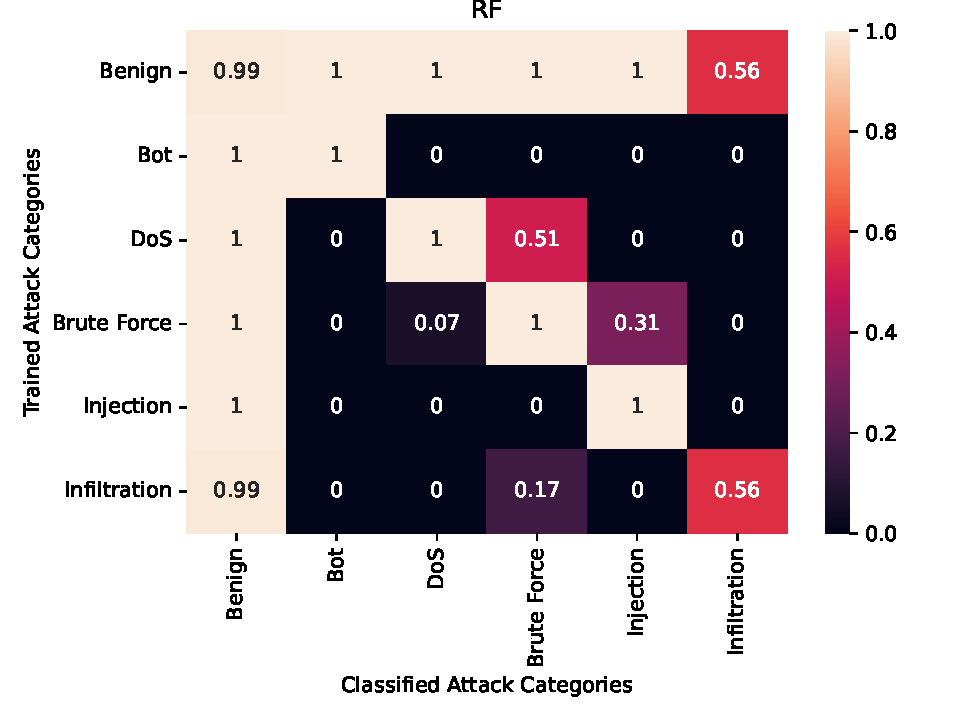
\includegraphics[width=\textwidth,keepaspectratio]{rf_inc_category}
    \end{minipage}
    %
    \begin{minipage}[h]{0.5\textwidth}
        \centering
        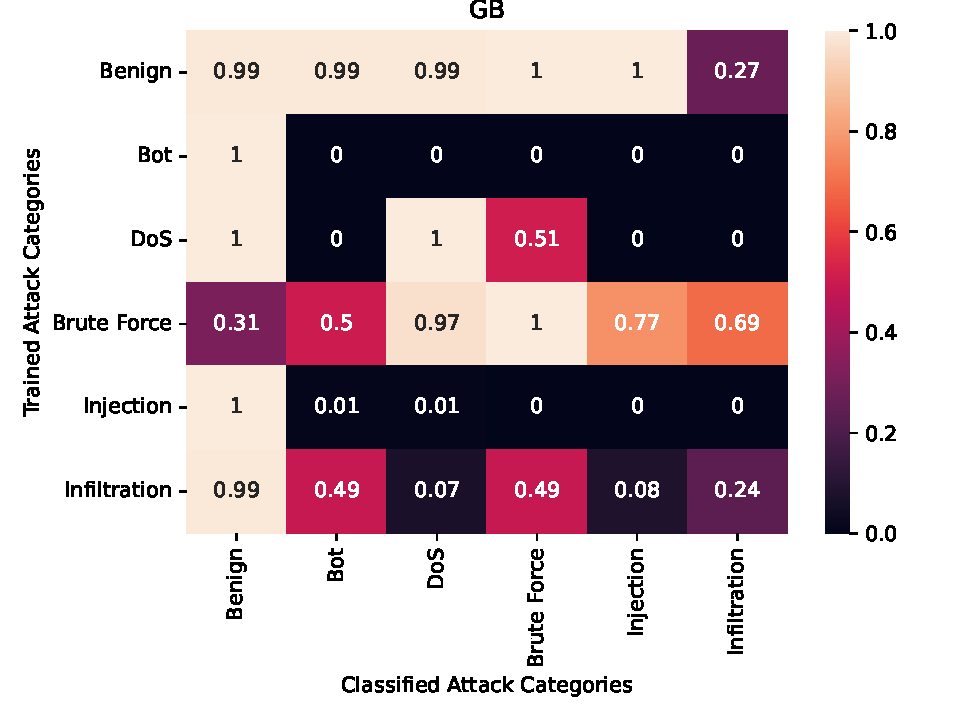
\includegraphics[width=\textwidth,keepaspectratio]{gb_inc_category}
    \end{minipage}\hfill
    \begin{minipage}[h]{0.5\textwidth}
        \centering
        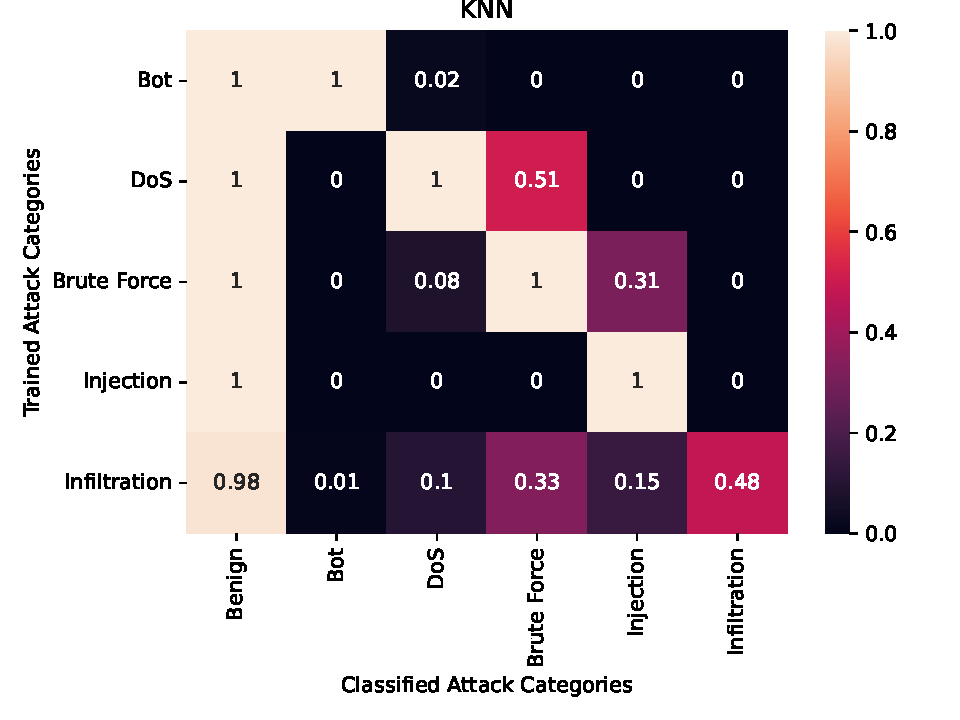
\includegraphics[width=\textwidth,keepaspectratio]{knn_inc_category}
    \end{minipage}
    \begin{minipage}[h]{0.5\textwidth}
        \centering
        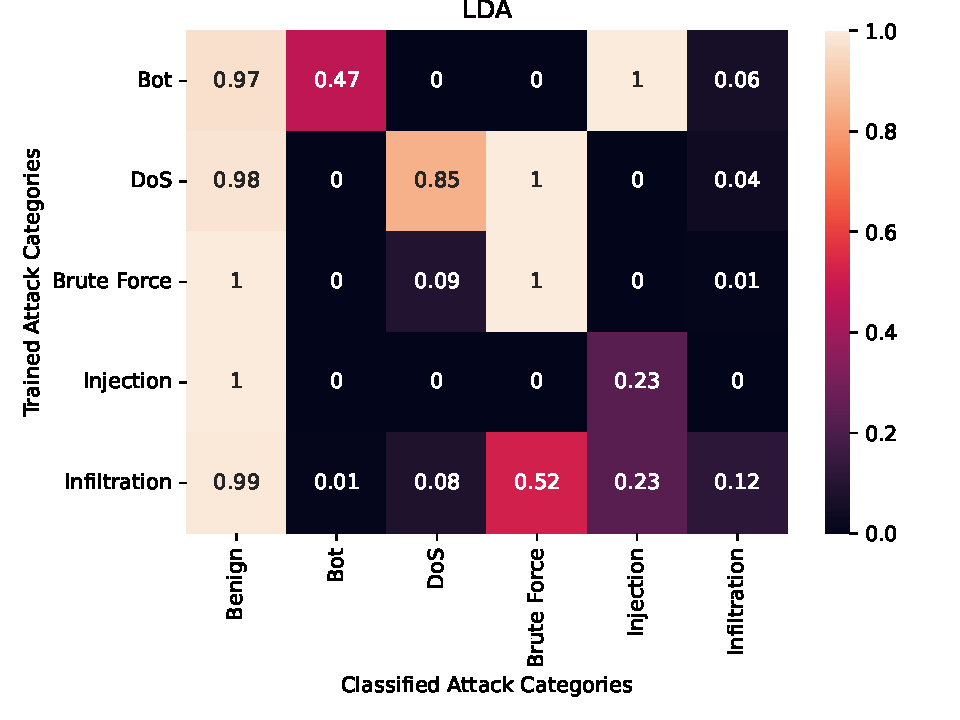
\includegraphics[width=\textwidth,keepaspectratio]{lda_inc_category}
    \end{minipage}
    \caption[Single Category Results]{Recall values per class when trained on a single category.\label{fig:inc_cat}}
\end{figure}
% 
This strange behaviour can be further explored in Figure~\ref{fig:inc_cat},
which shows the heatmaps of recall values generated from the variants including
single categories. The \gls{gb} algorithm seems to be able to learn patterns
that allow it to generalise from the Brute Force and Infiltration categories,
but fails to learn anything from the Bot and Injection categories.

The tree based algorithms are able to learn from all categories, indicated by
the high recall values in the diagonal. The \gls{dt} classifier also seems to
be able to generalise from the infiltration class. This behaviour, in
conjunction with the previous observations on the low accuracy on this class
supports the idea that the infiltration category may be too broad and contain
more than one sort of attack. This would explain why it is difficult to
classify, yet offers information about a wide variety of attacks.

Despite these limited instances of generalisation, the overall generalisation
ability of the three models is low. Most instances of generalisation on this
set of heatmaps yield low recall values, with the diagonal containing
significantly higher values indicating a limited ability to generalise across
categories.
%
\begin{figure}[htbp]
    \centering
    \begin{minipage}[h]{0.5\textwidth}
        \centering
        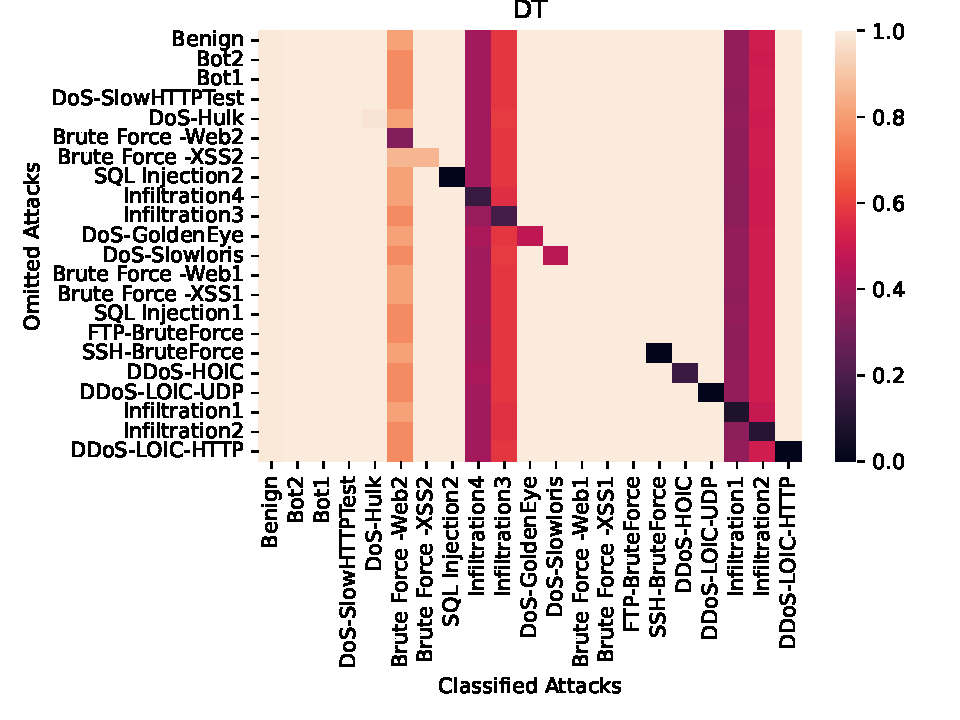
\includegraphics[width=\textwidth,keepaspectratio]{dt_exc_attack}
    \end{minipage}\hfill
    \begin{minipage}[h]{0.5\textwidth}
        \centering
        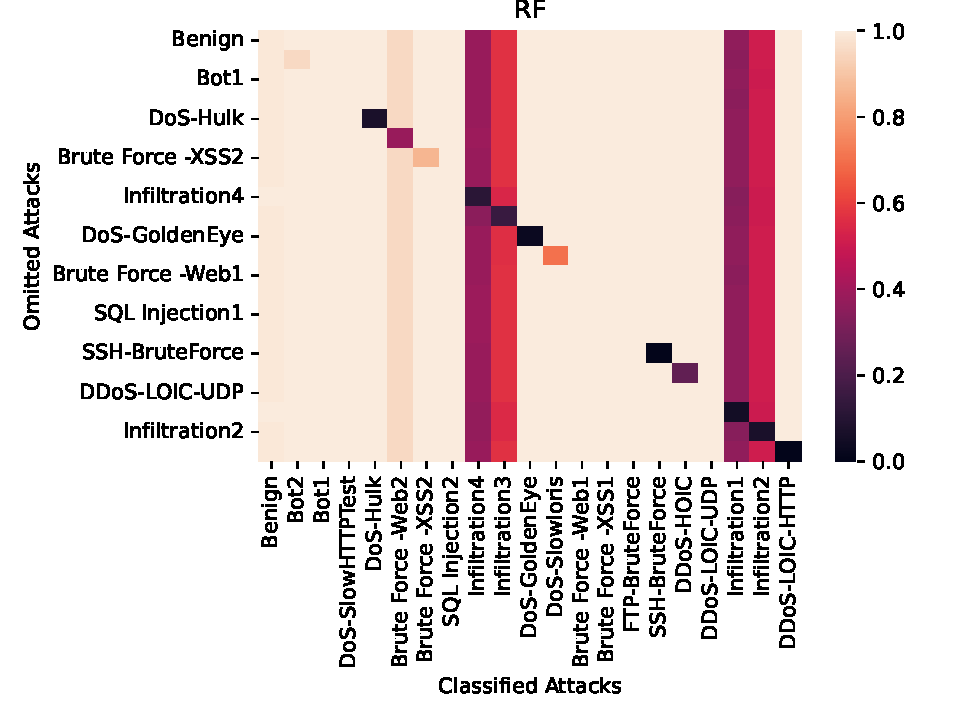
\includegraphics[width=\textwidth,keepaspectratio]{rf_exc_attack}
    \end{minipage}
    %
    \begin{minipage}[h]{0.5\textwidth}
        \centering
        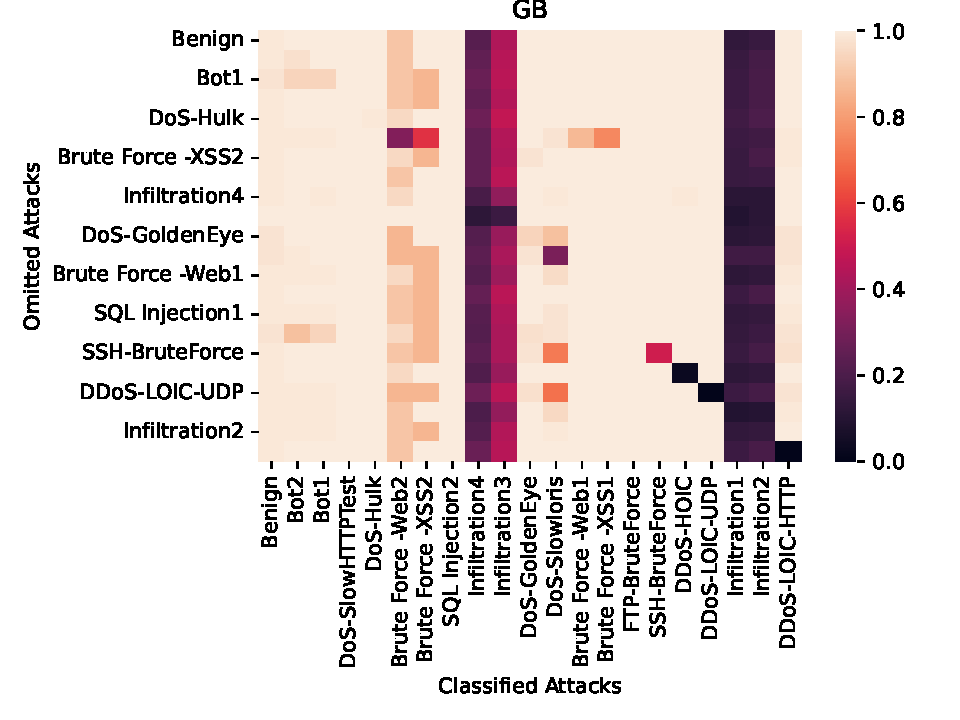
\includegraphics[width=\textwidth,keepaspectratio]{gb_exc_attack}
    \end{minipage}\hfill
    \begin{minipage}[h]{0.5\textwidth}
        \centering
        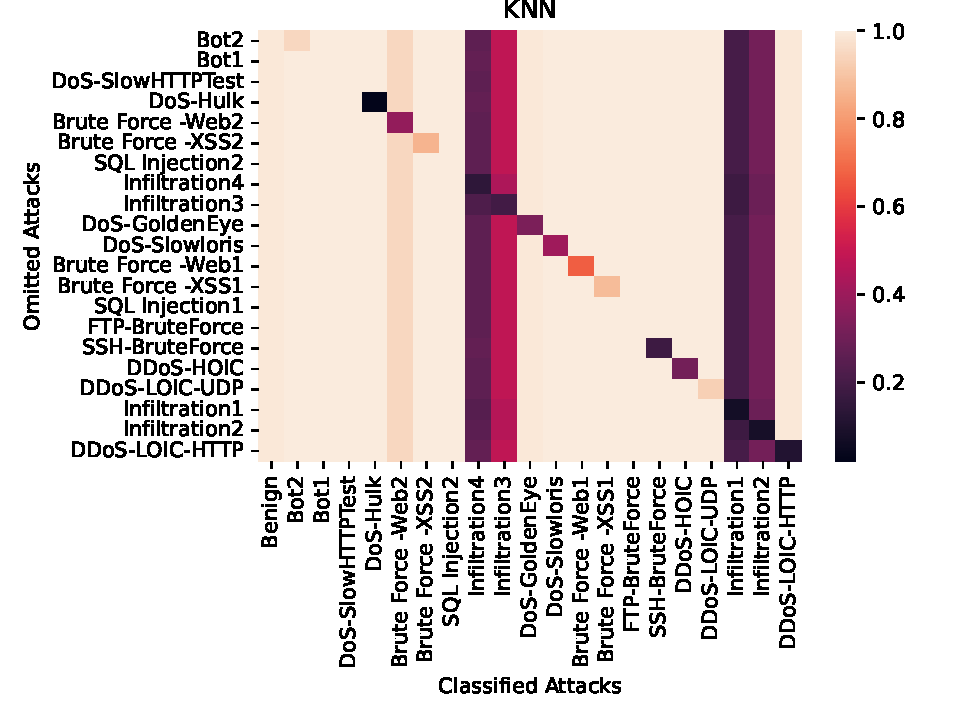
\includegraphics[width=\textwidth,keepaspectratio]{knn_exc_attack}
    \end{minipage}
    \begin{minipage}[h]{0.5\textwidth}
        \centering
        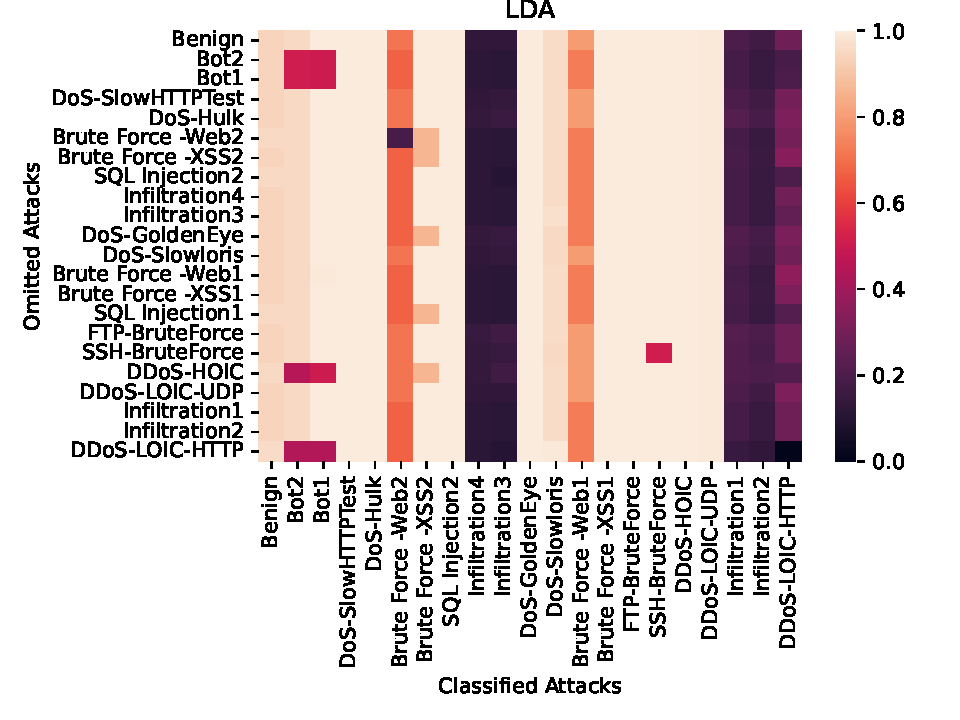
\includegraphics[width=\textwidth,keepaspectratio]{lda_exc_attack}
    \end{minipage}
    \caption[Individual Attack Omission Results.]{Recall values per class when trained on variants omitting a single attack.\label{fig:exc_att}}
\end{figure}
%
Figure~\ref{fig:exc_att} shows the heatmaps of recall values of the supervised
models generated from the variants omitting individual attacks. Each row
represents the per attack recall values generated from one variant. The label
of the row is the attack that was omitted.

The primary patterns to observe are the vertical stripes wherever infiltration
attacks are present and the diagonal, representing the difficulty of
classifying infiltration attacks and generalising to unknown attacks. It is
interesting to note, the diagonals have gaps, unlike in the category heatmaps.
This indicates intra-category generalisation occurs during training, creating
these gaps that are not visible in the category heatmaps. The slightly more
noisy heatmap resulting from the \gls{gb} algorithm is further evidence this
algorithm is more dependent on generalised patterns compared to the tree based
models.

\begin{figure}[htbp]
    \centering
    \begin{minipage}[h]{0.5\textwidth}
        \centering
        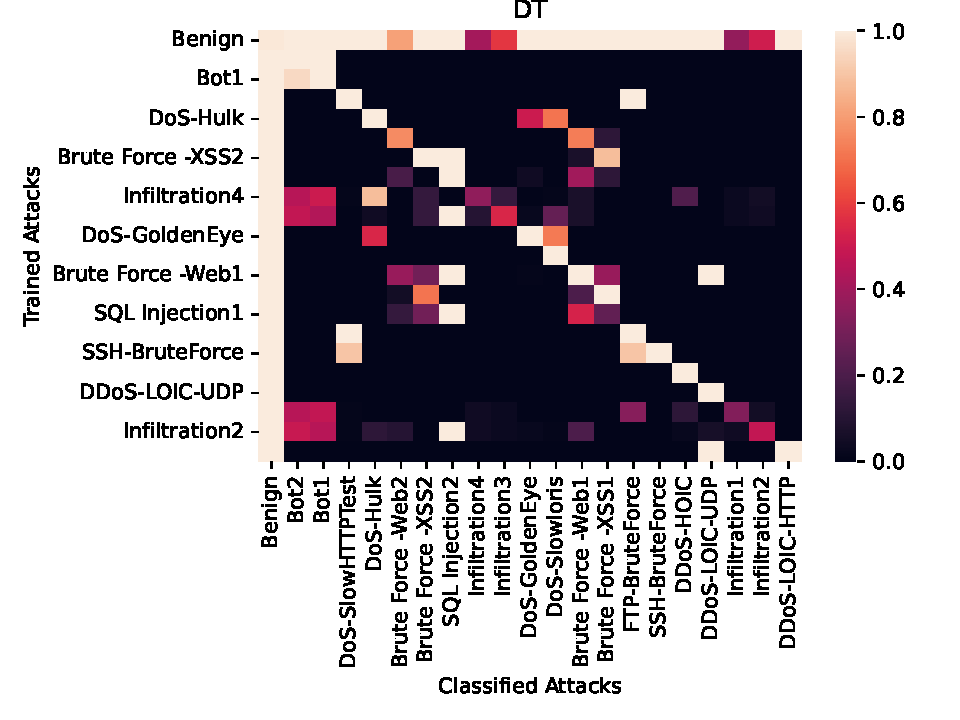
\includegraphics[width=\textwidth,keepaspectratio]{dt_inc_attack}
    \end{minipage}\hfill
    \begin{minipage}[h]{0.5\textwidth}
        \centering
        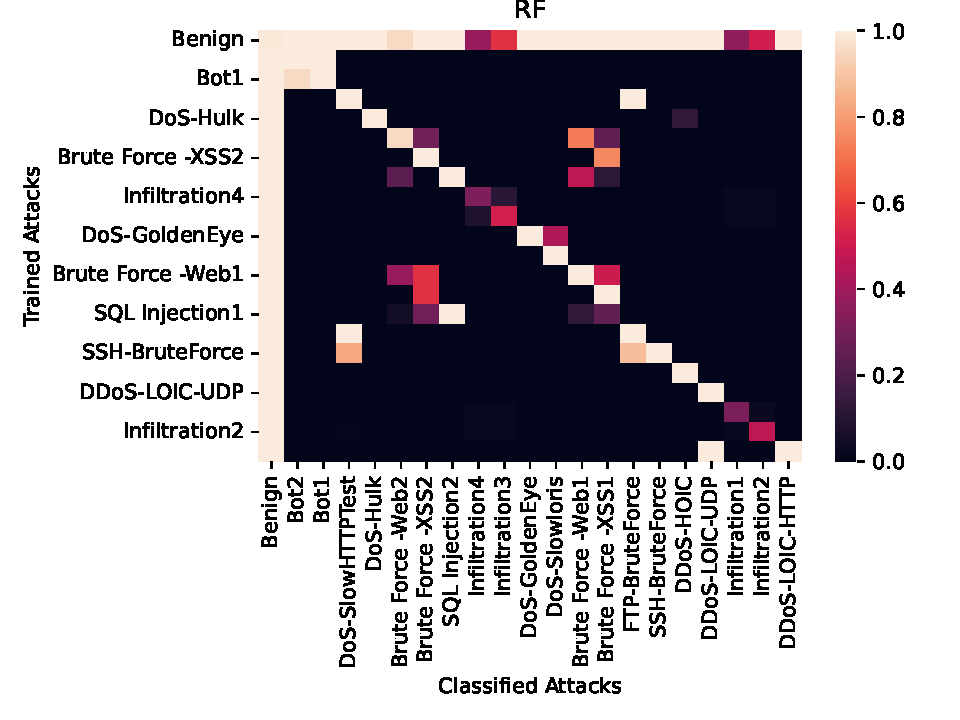
\includegraphics[width=\textwidth,keepaspectratio]{rf_inc_attack}
    \end{minipage}
    %
    \begin{minipage}[h]{0.5\textwidth}
        \centering
        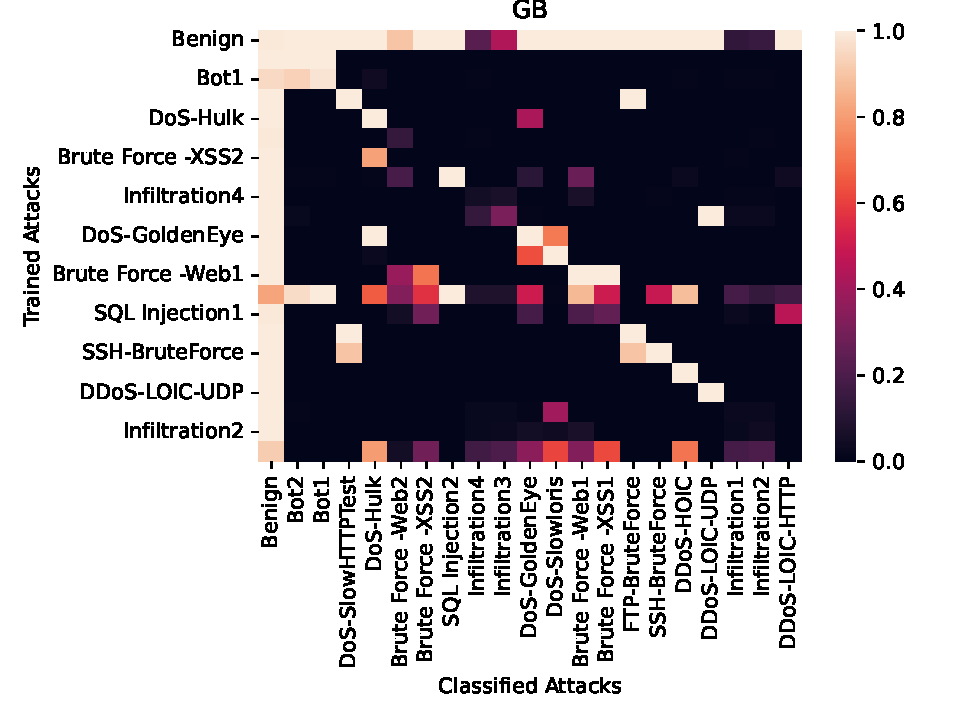
\includegraphics[width=\textwidth,keepaspectratio]{gb_inc_attack}
    \end{minipage}\hfill
    \begin{minipage}[h]{0.5\textwidth}
        \centering
        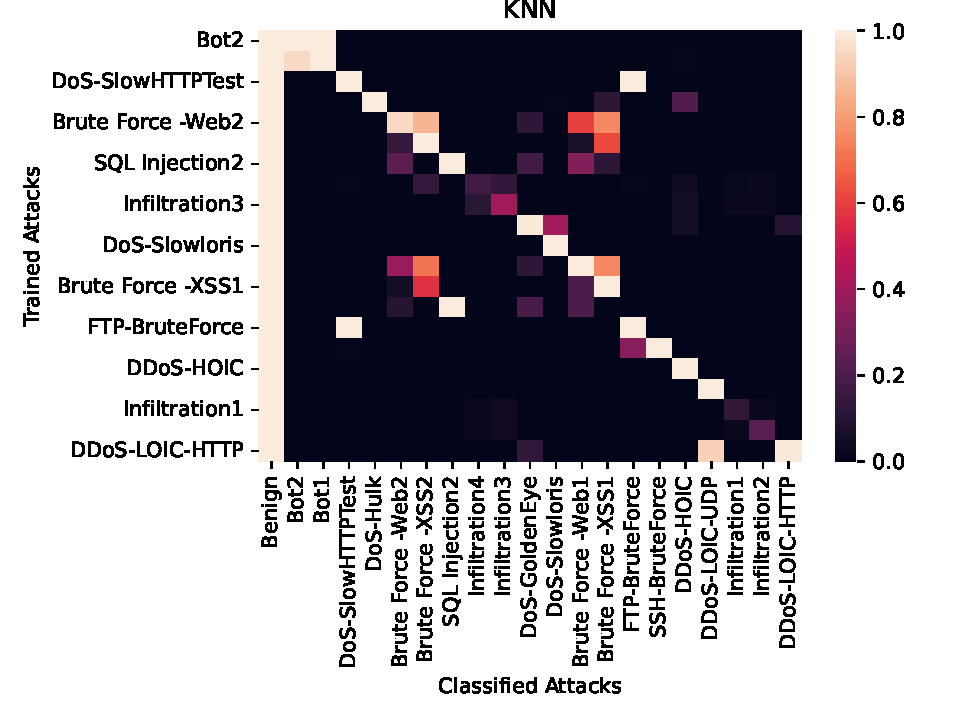
\includegraphics[width=\textwidth,keepaspectratio]{knn_inc_attack}
    \end{minipage}
    \begin{minipage}[h]{0.5\textwidth}
        \centering
        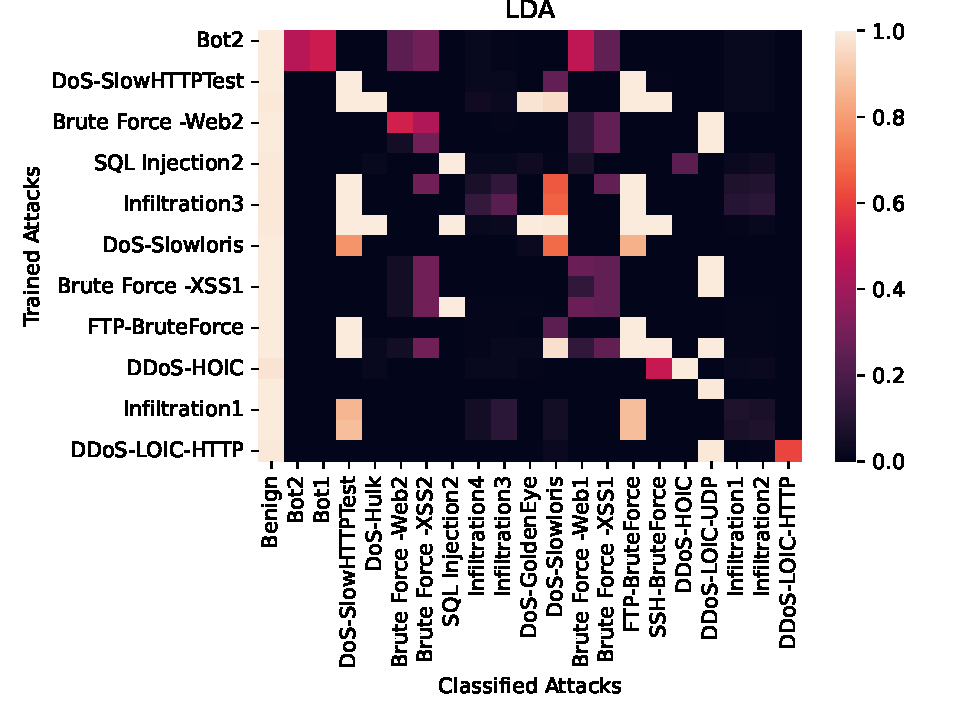
\includegraphics[width=\textwidth,keepaspectratio]{lda_inc_attack}
    \end{minipage}
    \caption[Single Individual Attack Results]{Recall values per class when trained on a single attack.\label{fig:inc_att}}
\end{figure}
%

Figure~\ref{fig:inc_att} shows the heatmaps of recall values generated from the
variants including single attacks. These results indicate that while
generalisation is somewhat scarce, there are numerous attacks in the dataset
that influence the model's performance on other attacks. The exact
relationships between each pair of attacks are indicated in the heatmaps. It
should be noted that the algorithm employed seems to have a significant effect
on the level of generalisation achieved, with \gls{gb} demonstrating the
highest generalisation ability, followed by \gls{dt} and finally \gls{rf}.

\section{Threats to Validity}%
\label{sec:threats}
% TODO, citations would take this up a notch
It should be noted from the results, that the \gls{sae}-\gls{ocsvm} model
performs much better on the NSL-KDD dataset than the CSE-CIC-IDS2018 dataset.
This highlights the issue of generalisation across datasets. The unsupervised
models considered were selected as they were the most highly cited and best
performing models within the domain that provide a clear methodology from the
models found during the literature review. This implicitly assumes that the
high efficacy demonstrated on the NSL-KDD dataset and the other datasets they
were evaluated on, generalises well to the CSE-CIC-IDS2018 dataset, which may
not always be the case. Hence, it is possible these models are not the best
performing models on the dataset considered for this study, resulting in an
unfair comparison with the supervised models.

Furthermore, the issue of cross-dataset generalisation also brings into
question how well these results will truly generalise outside the lab
environment. Whilst, to the best of our knowledge, the CSE-CIC-IDS2018 dataset
is the most up-to-date and realistic dataset currently available, it may still
not generalise well to other datasets and practical environments.

As mentioned in Section~\ref{sec:preprocessing} the individual attack labels
were generated based on the timestamp and label information in Table 2 of the
CSE-CIC-IDS2018 website~\cite{cic2018}. It was also mentioned that some attack
instances are dated outside the range of any attack listed on the table, and it
has therefore been assumed that instances occurring on a date with only one
attack of that label, belong to that attack. This assumption, whilst likely the
most logical approach, may lead to the mislabelling of certain samples.
Measuring the likelihood of this or mitigating the issues is difficult without
more information on the source of the ambiguous samples, which does not appear
to be available in the resources documenting the dataset.

As mentioned in Chapter~\ref{chp:evaluation}, the preprocessing took place
prior to the generation of dataset variants. The primary motivation for this
decision was the reduction of training time, which was necessary due to the
time constraints for this project. This means the preprocessing pipeline had
access to all the data, including the omitted samples. This has no effect
during most steps of preprocessing as most only consider values within the same
instance. The only exception to this is the handling of infinity values, which
involves taking the maximum value in the column and adding one. If the max
value belongs to an instance that will later be filtered out, it is possible
for omitted instances to influence instances that are not omitted during the
experiment. This effect is likely to be negligible, however still represents a
threat to validity.

Finally, all pragmatic cyberthreat defence systems present vulnerabilities of
their own which should be kept in mind when considering results. The
CSE-CIC-IDS2018 dataset was not designed with the \gls{nids} components
employed by this study in mind. Hence, the attacks it contains were performed
without any knowledge of the defence system we have employed. In practice,
attackers could learn implementation details of any defence system and
orchestrate targeted attacks intended to circumvent that specific defence
system. A prime example of such an attack targeted at \gls{ml}-based \gls{nids}
are adversarial attacks, which are attacks intentionally designed to evade
\gls{ml}-based classifiers.~\cite{adversarial1} and~\cite{adversarial2} propose
examples of such attack tools.
